% superlight clients
% sidechains
\section{Our Contributions}
\subsection{Superblocks}

We create a decentralized blockchain client or verifier which, having only
\emph{genesis}, connects to multiple provers, at least one of which is honest,
is able to ascertain the confirmation of a transaction. Using its full local
chain, each prover generates a succinct proof and sends it to the verifier.
Adversarial provers can send anything in the place of a proof. By comparing the
proofs in terms of the amount of proof-of-work they encode, the verifier deduces
which blockchain contains the most proof-of-work without receiving and
validating every block header. The proofs the provers send are only generated
once and do not require multiple interrogation questions from the verifier. As
such, these proofs are non-interactive and we call them \emph{Non-Interactive
Proofs of Proof-of-Work} (NIPoPoWs).

To create such succinct representations of work, we look at the distribution of
block hashes in the chain. Every valid block $B$ satisfies the proof-of-work
equation $H(B) \leq T$ where $T$ is the mining target, but some blocks satisfy
it better than others. Some blocks so happen to have a hash with value
\emph{much} lower than $T$, even though this is not required for validity and is
not intentional. For example, some blocks will satisfy $H(B) \leq \frac{T}{2}$.
Concretely, because the hash function is uniformly distributed, in expectation
\emph{half} the blocks will satisfy $H(B) \leq \frac{T}{2}$, a \emph{quarter} of
them will satisfy $H(B) \leq \frac{T}{4}$, an \emph{eighth} will satisfy $H(B)
\leq \frac{T}{8}$, and in general only a $\frac{1}{2^\mu}$ fraction of blocks
will satisfy $H(B) \leq \frac{T}{2^\mu}$. If a block satisfies this inequality
for some $\mu \in \mathbb{N}$, we say that it is of \emph{level} $\mu$ and call
it a $\mu$-superblock (and note that a $\mu$-superblock for $\mu > 0$ is also
a $(\mu - 1)$-superblock). The probability of a valid block $B$ being a
$\mu$-superblock is:

\[
\Pr[H(B) \leq \frac{T}{2^\mu}|H(B) \leq T] = \frac{1}{2^\mu}
\]

Under this light, the blockchain looks as illustrated in
Figure~\ref{fig.superblocks}. Of course, because block hashes behave randomly,
this image will be probabilistic and blocks may not be precisely distributed as
expected.

\begin{figure}[ht]
    \caption{Superblocks distributed within a blockchain.
    Higher levels have achieved a higher difficulty during
    mining.}
    \centering
    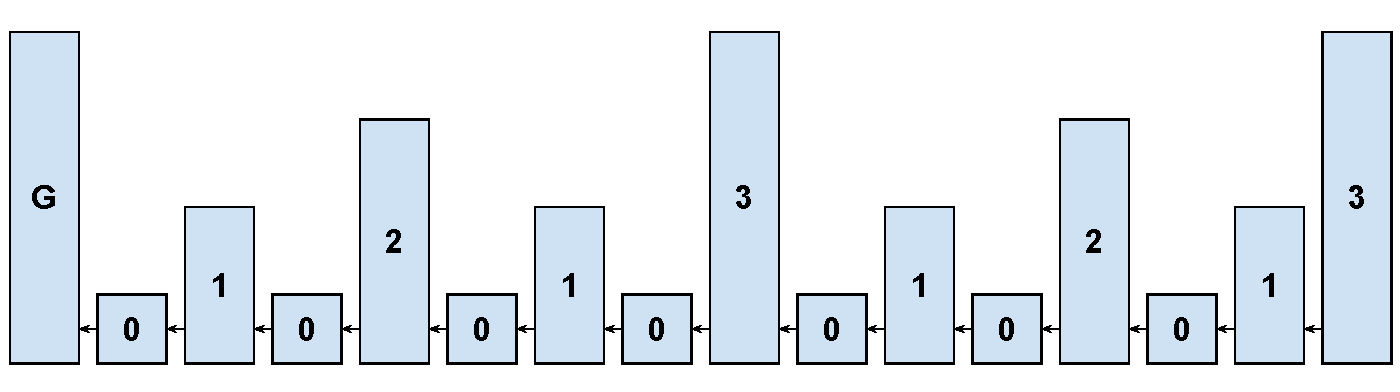
\includegraphics[width=0.7\columnwidth,keepaspectratio]{chapters/introduction/figures/superblocks.pdf}
    \label{fig.superblocks}
\end{figure}

The algorithm for this construction is shown in
Algorithm~\ref{alg.interlink-set}~\cite{compactsuperblocks}. The
interlink set of the Genesis block is, by definition, empty. The algorithm
describes how the interlink can be updated once a block is found. The new
interlink is then included in the next block. This construction ensures that
every block contains a direct pointer to its most recent $\mu$-superblock
ancestor, for every $\mu \in \mathbb{N}$.

\import{./}{chapters/superlight/algorithms/alg.interlink-set-update.tex}

The \textsf{updateInterlinkSet} algorithm accepts a block $B'$, which already has an
interlink data structure defined on it. The function evaluates the
interlink data structure which needs to be included as part of the next block.
It copies the existing interlink data structure from level $\textsf{level}(B')$
and adds the reference $H(B')$.
\todo{continuity}

\todo{NIPoPoWs}
\todo{applications to superlight wallets}
\todo{applications to sidechains}
\todo{applications to logspace mining}
\todo{the variable difficulty and $\Delta$-delay setting}
\todo{proofs of stake}

\ifdraft
\todo{Clean up paragraph}
In this section, we introduce the first
trustless construction for proof-of-work sidechains. We describe how to build
generic communication between blockchains. As one application, we give the
construction of a \emph{two-way pegged} asset which can be moved from one
blockchain to another while retaining its nature. We provide a high-level
construction in Solidity. Our construction works across a broad range of
blockchains requiring only two underlying properties. First, that the
\emph{source} blockchain is a proof-of-work blockchain supporting
Non-Interactive Proofs of Proof-of-Work (NIPoPoWs), a cryptographic primitive
which allows constructing succinct proofs \emph{about} events which occur in a
proof-of-work blockchain and which was recently introduced in~\cite{nipopows}.
Support for NIPoPoWs can be introduced to practically any
work-based cryptocurrency such as Bitcoin and Ethereum without a hard or soft
fork. Second, that the \emph{target} blockchain is able to validate such proofs
through smart contracts such as, e.g., Ethereum or Ethereum
Classic.
We give a formal proof of security of our construction via
reduction to NIPoPoW security under the assumption that the interoperating
blockchains are secure individually.
To our knowledge, we are the first to
provide such a construction in
full and prove its security.
\fi

\subsection{Summary of Contributions}
A summary of our contributions and their dependencies, with annotations
indicating where they are presented in this thesis, is visually illustrated in
Figure~\ref{fig.contributions}.

In summary, in this thesis we solve the problem of \emph{consensus compression}
for all decentralized blockchain consensus mechanisms. \textbf{For
proof-of-work}, we introduce the NIPoPoWs primitive (Chapter 3) and we give two
superblock-based constructions of succinct NIPoPoWs protocols in the Backbone
model: First the \emph{charity} construction (Chapter~\ref{chapter:work}), and
second the \emph{distill} construction (Chapter~\ref{chapter:variable}
and~\ref{chapter:superlight}). In the static synchronous model
(Chapter~\ref{chapter:work}), we prove our charity construction with
\emph{goodness} secure against $\frac{1}{2}$ adversaries, but succinct only in
the optimistic setting. Our charity construction \emph{without goodness} as well
as our distill construction are both secure and succinct against $\frac{1}{3}$
adversaries (Chapter~\ref{chapter:variable}). In the synchronous variable model
(Chapter~\ref{chapter:variable}), our distill construction is secure against a
$\frac{1}{3}$ adversary as long as difficulty is non-decreasing. Our charity
without goodness construction is secure against a $\frac{1}{3}$ adversary even
if difficult is not limited to non-decreasing. Both are succinct as long as
difficulty is not exponentially decreasing. Lastly, in the $\Delta$-bounded
delay setting (Chapter~\ref{chapter:variable}), both constructions are secure
and succinct under the same limitations, but only against a $\frac{1}{4}$
adversary. We give concrete parameter recommendations and run experiments and
simulations indicatively for the charity construction of
Chapter~\ref{chapter:work}. \textbf{For proof-of-stake}, we construct the ATMs
primitive and give signature-based construction (Chapter~\ref{chapter:stake}).
These are secure in the Ouroboros model, but offer only constant improvements
over full clients and hence do not achieve asymptotic succinctness.

We make use of these primitives to build \textbf{cross-chain transfer}
applications, which give rise to interoperability among blockchains, allowing
generic information transfer among work/work, work/stake, and stake/stake
chains. We give the definition of what constitutes a secure sidechain protocol
(Chapter~\ref{chapter:sidechains}) and put forth cross-chain protocols which we
prove secure. Our protocols can work natively or by leveraging smart contract
functionality. We show how they can be utilized to create one-way and two-way
pegs and discuss several deployment mechanisms which allow them to be deployed
as soft forks or better. Our protocols can also be used to build superlight
clients. Lastly, we show that our proof-of-work protocols specifically can be
utilized to build logarithmic-space miners (Chapter~\ref{chapter:superlight}),
providing exponential improvements over the state and communication complexity
of existing blockchain protocols.

\begin{figure}
    \caption{
      A roadmap of this thesis' structure.
      Our underlying model is shown above the double line.
      Our contributions are shown below the double line and comprise consensus
      compression primitives (above the dashed line) and their applications
      (below the dashed line). The respective chapters are indicated next to
      each topic.
    }
    \centering
    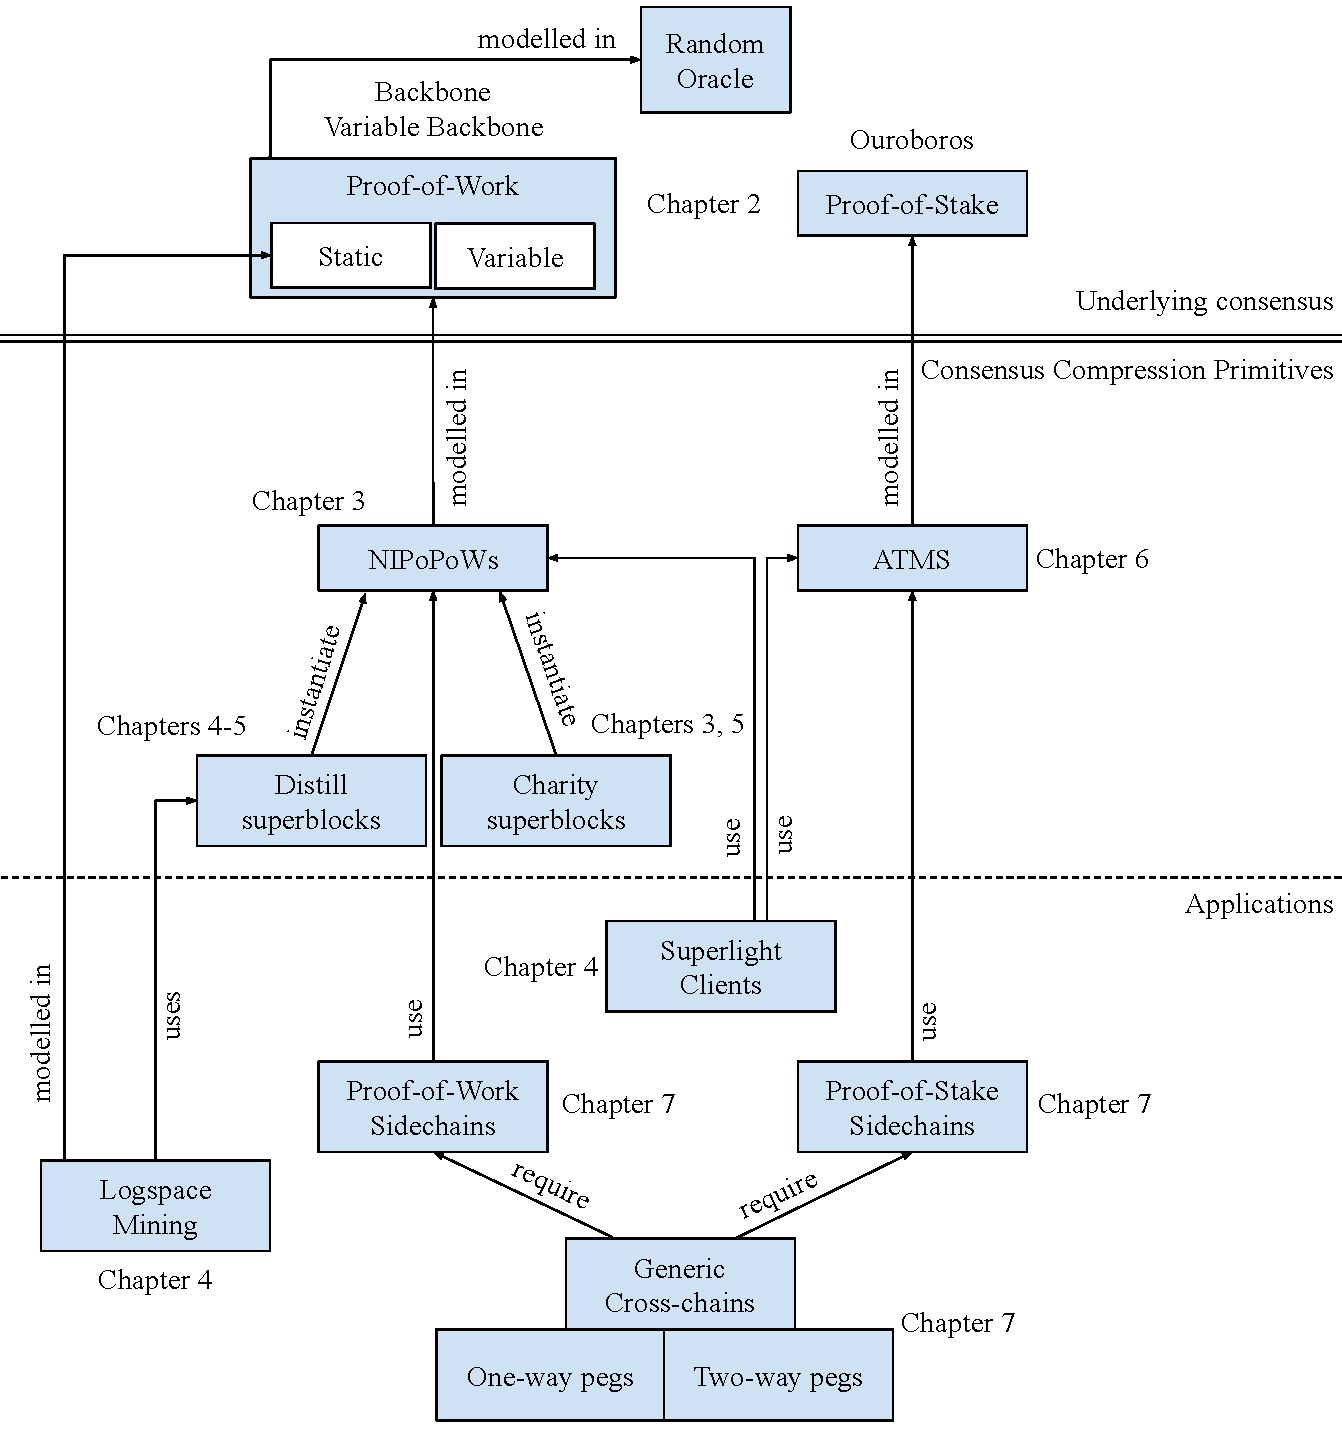
\includegraphics[width=\columnwidth,keepaspectratio]{chapters/introduction/figures/contributions.pdf}
    \label{fig.contributions}
\end{figure}
